\documentclass{article}
\usepackage{polski}
\usepackage[utf8]{inputenc}
\usepackage{mathtools}
\usepackage{amsmath}
\usepackage{amssymb}
\usepackage{tabulary}
\usepackage{booktabs}
\usepackage{graphicx}
\usepackage{xcolor}
\usepackage[a4paper, margin=1.5cm]{geometry}

\graphicspath{ {images/} }

\title{Wirtualizacja zasobów oraz alokacja przepływów w sieciach sterowanych programowo przy jednoczesnym zapewnieniu wymagań QoS}
\author{
  Chodacki, Maksymzilian\      \texttt{maksymilian.chodacki@gmail.com}
  \and
  Grzanka, Antoni\      \texttt{antoni.grzanka@gmail.com}
  \and
  Leniart, Eryk\      \texttt{eryk.leniart@gmail.com}
  \and
  Niedziałkowski, Adam\      \texttt{adam.niedzialkowski@gmail.com}
}
\date{17 Stycznia 2017}

\begin{document}

\maketitle

\section{Wstęp}

Sieci sterowane programowo (SDN, z ang. Software Defined Networks) to koncept, który coraz bardziej zyskuje na wadze w dzisiejszym świecie architektury systemów i sieci. Koncepcja oddzielenia warstwy kontrolującej sieć od mechanizmów związanych z transmisją danych rozwiązuje wiele problemów, przed którymi stają codziennie architekci sieci. Jednym z wyzwań, przed którym stają operatorzy chcący zaimplementować w swojej sieci mechanizm SDN jest sprawiedliwy podział zasobów pomiędzy swoich klientów (dzierżawców) oraz zapewnienie takiej alokacji przepływów, która zapewni płynne działanie sieci. Jest to krytycznie ważna kwestia, ponieważ w rzeczywistych zastosowaniach, każdy z klientów (dzierżawców) sieci ma swoje wymagania odnośnie świadczonych przez operatora usług, których niespełnienie może wiązać się z poważnymi konsekwencjami finansowymi. Do tego typu parametrów zaliczamy jitter, opóźnienie przesyłu czy utratę pakietów. \newline

\noindent W pracy \cite{lin16} autorzy proponują kompleksowe rozwiązanie powyższego problemu, obejmujące dwustopniowy model optymalizacyjny (wirtualizacja zasobów poprzez podział sieci oraz maksymalizacja minimalnego przepływu).  \newline

\noindent W poniższej pracy autorzy skupili się na optymalizacji sposobu alokacji przepływów względem innych parametrów niż te zaproponowane w \cite{lin16}, co może bardziej realistycznie odpowiadać zapotrzebowaniom klientów. W tym celu przeanalizowano algorytm zaproponowany w \cite{lin16}, dokonano jego implementacji w języku ILOG, a także rozszerzono go, proponując dwa alternatywne modele ostatniej fazy działania algorytmu.

\section{Wykorzystywane symbole}

Stałe i indeksy:
\begin{tabular}{l l}
$N$ & zbiór $|N|$ dzierżawców \\
$n$ & pojedynczy dzierżawca, $n \in N$ \\
$F$ & zbiór $|F|$ zdefiniowanych przepływów \\
$f$ & pojedynczy przepływ, $f \in F$ \\
$E$ & zbiór $|E|$ łącz \\
$E^f_n$ & zbiór $|E|$ łącz należących do przepływu $f$ dla dzierżawcy $n$\\
$e = (i,j)$ & pojedyncze łącze rozpoczynające się w węźle $i$ kończące się w węźle $j$, $e \in E$ \\
\end{tabular}

Zmienne decyzyjne:
\begin{tabular}{l l}
$x_{an}$ & zmienna w modelu podziału zasobów \\
\end{tabular}

\section{Podział zasobów}

Pierwszą częścią algorytmu zaproponowanego w [1] jest podział sieci pomiędzy dzierżawców (klientów) tak, aby możliwie ich od siebie odizolować. Dopiero na tak przygotowanej, podzielonej sieci dokonuje się alokacji przepływów oraz sprawdzenia wymagań dotyczących parametrów Quality of Service. \newline

Celem optymalizacji w pierwszym modelu jest maksymalna izolacja infrastruktury wykorzystywanej przez różnych dzierżawców, co można osiągnąć np. przez minimalizację łącz współdzielonych przez różnych klientów:

\begin{equation}
  \min \sum_{n_{1} \in N} \sum_{n_{2} \in N} \sum_{e \in E} x_{en_{1}} x_{en_{2}}
\end{equation}

W celu zapewnienia łączności każdego z węzłów z dowolnym innym dodano ograniczenia powodujące zbudowanie drzewa rozpinającego na grafie:

\begin{equation}
  \forall_{n \in N} \sum_{e \in E} x_{an} \ge N-1
\end{equation}

\begin{equation}
  \forall_{n \in N} \forall_{Z \in V: Z \subset V, Z \neq \emptyset } \sum_{e \in S_{n}} x_{en} \ge 1
\end{equation}

gdzie $Z$ to zbiór podgrafów $V$ a $S_{n}$ to zbiór wszystkich łącz mających swój początek w $Z$ a koniec w $V \setminus Z$. Powyższe ujęcie problemu zbudowania drzewa rozpinającego znane jest jako \textit{cutset formulation} i zapewnia, że w każdym zbudowanym drzewie wszystkie węzły będą miały łączność z dowolnym innym.

Z uwagi na to, że implementacja wymagała wykorzystania dwóch łącz dla każdego połączenia, należało dodać również ograniczenie zabraniające jakiemukolwiek dzierżawcy korzystanie z łącza tylko w jedną stronę:

\begin{equation}
  \forall_{n \in N} \forall_{Z \in V: Z \subset V, Z \neq \emptyset } \forall_{e \in S_{n}} x_{en} = x_{e'n}
\end{equation}

gdzie ${e'}$ symbolizuje łącze komplementarne do ${e}$ łączące te same węzły w drugą stronę, tj. $\forall_{e \in E: e = (i,j)} \exists_{e' \in E: e' = (j,i)}$.

\section{Model alokacji przepływu}

Naszym kolejnym krokiem było zaimplementowanie modelu alokacji przepływów, w
którym funkcją celu jest maksymalizacja minimalnego przepływu, czyli zrównoważenie
ruchu generowanego przez przepływy dzierżawców na wszystkie dostępne łącza:

\begin{equation}
  \sum_{n \in N} \max_{\{X_{f,i,j}^n;\forall{(i,j)} \in E_n^f,f \in F^n\}} \min_{f \in F^n}\lambda_f^n
\end{equation}

W modelu zostało zaimplementowanych pięć ograniczeń. Pierwsze z nich zapewnia,
że suma wartości przepływów na danym łączu nie przekroczy jego pojemności:

\begin{equation}
  \sum_{n \in N} \sum_{f \in F^n} X_{f,i,j}^n \le c_{ij}
\end{equation}

Kolene ograniczenie nazywane konserwacją przepływów zapewnia, że dla danego węzła
niebędącego węzłem docelowym, dla dowolnego przepływu suma wartości wychodzących
przepływów jest równa sumie wartości przychodzących przepływów plus wartość danego
przepływu jeśli jest to węzęł źródłowy dla tego przepływu. W innym wypadku suma ta
równa się zero:

\begin{equation}
\begin{align*}
  \sum_{j;(i,j) \in E_n^f} X_{f,i,j}^n &- \sum_{j;(j,i) \in E_n^f} X_{f,i,j}^n = \lambda_f^n \parallel_{\{i=s_f^n\}} \\
  & \forall{i} \ne d_f^n, f \in F^n, n \in N
\end{align*}
\end{equation}

Następne ograniczenie zapewnia, że przepływ nie może zostać rozdzielony na
dwa lub więcej łączy:

\begin{equation}
  X_{f,i,j}^n = 0 \quad \forall(i,j) \notin E_n^f, f \in F^n, n \in N
\end{equation}

Czwarte ograniczenie związane jest z zapewnieniem jakości obsługi. Wymusza ono, że
iloczyn straty pakietów na łączach przypisanych do danego przepływu nie przekroczy
ustalonej maksymalnej wartości:

\begin{equation}
  \prod_{(i,j) \in E_n^f} p_{f,i,j}^n < p_{n,f}^{max}
\end{equation}

Ostatnie ograniczenie nie jest opisane przez autorów, zostało dodane przez nas
na potrzeby naszej struktury danych wejściowych, a dokładniej podzielonego grafu pomiędzy
dzierżawców. Ograniczenie to zapewnia, że dla danego dzierżawcy, każdy jego przepływ
nie będzie wykorzystywał łącz, które do niego nie należą:

\begin{equation}
  \forall_{f \in F^n} X_{f,i,j} = 0 \quad \text{jeśli}\quad x_{i,j}^f = 0
\end{equation}

\section{Główny skrypt}

//TODO: Eryk

\section{Testy}
Implementację opisanych wcześniej modeli testowaliśmy na trzech różnych topologiach - małej, średniej oraz
dużej. Początkowo sprawdzaliśmy działanie modeli oraz skryptu tylko na bardzo małej topologii. Było taki
ze względu na możliwość szybkiej weryfikacji poprawności działania kodu, a przy większych
topologiach nie bylibyśmy w stanie jednoznacznie określić czy dany model działa tak, jak zakładaliśmy.
\newline \newline
Testowanie polegało na sprawdzaniu czy zostały spełnione zakładane przez nas wcześniej warunki. Początkowo
były to sprawdzenie, czy każdy z dzierżawców posiada połączenie do wszystkich węzłów oraz czy liczba
wspólnych krawędzi dla wszystkich dzierżawców jest jak najmniejsza. Stopień trudności w weryfikowaniu
poprawności rozwiązania rósł wraz z każdym dodamym dzierżawcą, węzłem lub połączeniem, dlatego większość
testów przeprowadziliśmy dla topologii składającej się z sześciu węzłów, dwóch dzierżawców i ośmiu połączeń.
Była ona na tyle rozbudowana, że na pewnych etapach projektu pojawiały się błędy w działaniu naszych modeli,
a z drugiej strony na tyle przejrzysta, że byliśmy w stanie w niedługim czasie zweryfikować poprawność działania
modeli.
\newline \newline
Na podstawie przeprowadzonych testów stwierdzamy, że nasza implementacja działa w ten sam sposób,
w jaki zamierzaliśmy. Partycjonowanie sieci odbywa się prawidłowo - nie zdarza się, aby któryś z dzierżawców
nie miał dostępu do któregoś z węzłów. Liczba wspólnych krawędzi jest najmniejsza z możliwych - tutaj pewność
dobrego działania mamy tylko dla mniejszych topologii, w których byliśmy w stanie ręcznie sprawdzić wszystkie
możliwości i określić minimalną liczbę wspólnych krawędzi. Kolejną testowaną funkcjonalnością było
przydzielanie łączy do konkretnych przepływów. Sprawdzaliśmy, czy przez każde łącze płynie taki ruch, który
będzie w stanie się w nim zmieścić bez strat wynikających z jego łącza -
ten warunek także był spełniony dla naszych przypadków testowych.

\section{Rozszerzenie}

Po zaimplementowaniu podstawowego modelu postanowiliśmy podejść do tematu
rozszerzenia problemu na dwa sposoby: dodaniu nowych ograniczeń
oraz zastosowaniu go w innej formie. Zaproponowanym przez nas ograniczeniem jest
zapewnianie minimaalnej wartości przepływu, a nowym zastosowaniem jest wprowadzenie
kosztu jako głównej metryki optymalizacji sieci.

\subsection{Zapewnienie minimalnych wartości przepływu}

Istotnym aspektem nie poruszanym przez autorów pracy jest zapewnienie
minimalnej wartości przepływu. Autorzy odnieśli się do problemu zapewnienia wszystkim
przepływom dodatniej wartości (w praktyce wszystie przepływy będą miały równą wartość).
Pozwala to na sprawiedliwy podział zasobów, natomiast w przypadku jeżeli różnym
przepływom chcemy zapewnić różne minimalne wartości potrzebne jest rozszerzenie problemu
o nowe dane (minimalną liczbę danych dla każdego przepływu) oraz dodatkowe ograniczenie:

\begin{equation}
  \forall_{t \in T} \forall_{f \in F_t} \quad \lambda_{tf} \ge f.minimal
\end{equation}

\subsection{Koszt przesyłu danych}

W przypadku nowego zastosowania postanowiliśmy postawić na praktyczne podejście;
rozszerzylismy model o koszt przesyłanych danych i zmieniliśmy funkcję celu tak,
by zrównoważyć koszt przepływów:
\begin{equation}
  \sum_{t \in T} \max_{f \in F_t} \sum_{a \in A_f} a.cost
\end{equation}

\subsection{Wyniki roszerzonych modeli}
Poniżej przedstawiamy porównanie wyników modeli rozszerzonych i podstawowego wyliczonych
w środowisku CPLEX. Tabela zawiera wyniki dla trzech zestawów danych: sieci małej (4 hosty),
średniej (6 hostów) i dużej (17 hostów).

\section{Podsumowanie}
W opisanym projekcie skupiliśmy się na problemie optymalizacji sieci przy użyciu algorytmów zaproponowanych
przez azjatyckich naukowców. Udało nam się zaimplementować ich rozwiązanie i sprawdzić, czy rzeczywiście ono
działa. Założeniem projektu była minimalizacja liczby wspólnych łączy dzielonych przez kilku dzierżawców. Uzyskane
wyniki pozwalają nam stwierdzić, że projekt został zrealizowany poprawnie, spełnia wszystkie pierwotne założenia.
W trakcie problemu zmierzyliśmy się z kilkoma niebanalnymi problemami - jak na przykład linearyzacja ograniczeń,
przez co musieliśmy poświęcić na zrobienie projektu więcej czasu niż zakładaliśmy, z drugiej strony jednak mieliśmy
okazję więcej się nauczyć.



\begin{thebibliography}

\bibitem{lin16}
  Lin, Shih-Chun and Wang, Pu and Luo, Min,
  \emph{Jointly Optimized QoS-aware Virtualization and Routing in Software Defined Networks},
  Comput. Netw. Vol. 96,
  Elsevier North-Holland, Inc.
  February 2016.

\end{thebibliography}

\newpage
\section{Załącznik - wizualizacja wykorzystywanych topologii}

\subsection{Mała topologia}
\begin{minipage}{\linewidth}% to keep image and caption on one page
\makebox[\linewidth]{%        to center the image
  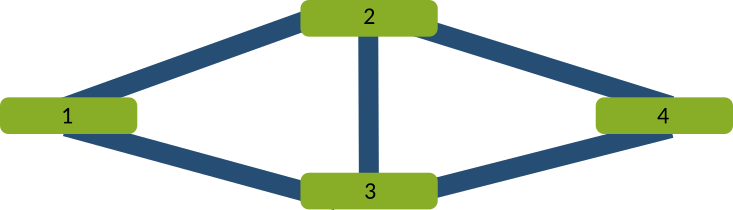
\includegraphics{topo1.png}}
\end{minipage}

\subsection{Średnia topologia}
\begin{minipage}{\linewidth}% to keep image and caption on one page
\makebox[\linewidth]{%        to center the image
  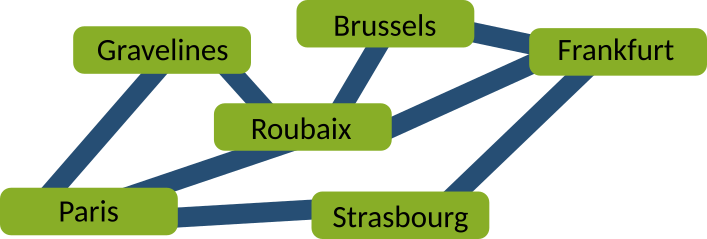
\includegraphics{topo2.png}}
\end{minipage}

\subsection{Duża topologia}
\begin{minipage}{\linewidth}% to keep image and caption on one page
\makebox[\linewidth]{%        to center the image
  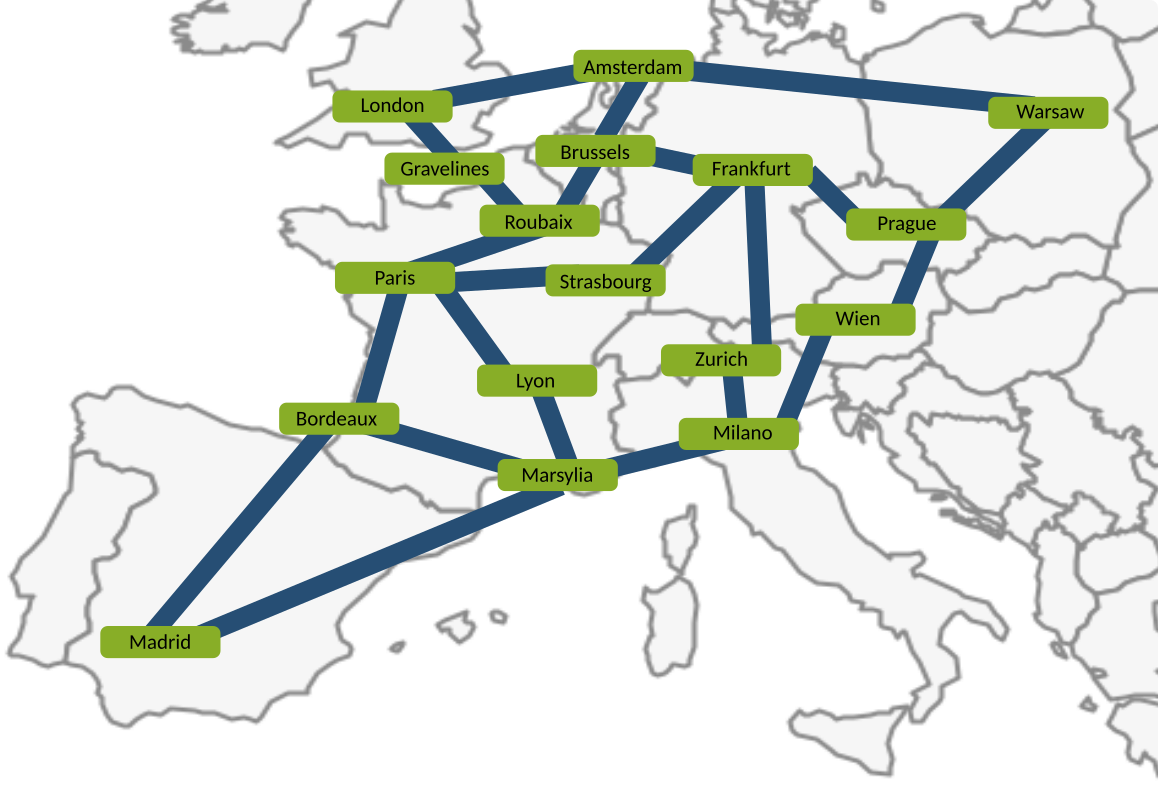
\includegraphics{topo3.png}}
\end{minipage}


\end{document}
